\documentclass[9pt, aspectratio=169]{beamer}
%\documentclass[9pt, aspectratio=169, handout]{beamer}

\usetheme{metropolis}
\setbeamertemplate{itemize items}{\faAngleRight}

\metroset{titleformat=smallcaps,block=fill,numbering=counter,progressbar=frametitle,sectionpage=none}
\setbeamersize{text margin left=5mm,text margin right=5mm} 
% \input{embed_video}
\usepackage{fontspec,minted}
\usepackage[scale=1]{ccicons}
\usepackage{metalogo}
\usepackage{xcolor,colortbl}
\usepackage{multicol,multirow,booktabs}
\usepackage{appendixnumberbeamer}
\usepackage{graphicx}
\usepackage{mismath}
\usepackage{bm}
\usepackage{fontawesome5}
\usepackage{csquotes}
%\usepackage[backend=biber, natbib, sorting=nyt, doi=true, url=false, url=false, isbn=false, maxbibnames=10]{biblatex}
%\addbibresource{../../utils/refs.bib}

\usepackage[spanish, es-nodecimaldot]{babel}
\deftranslation[to=spanish]{Definition}{Definición}
\deftranslation[to=spanish]{Theorem}{Teorema}
\deftranslation[to=spanish]{Example}{Ejemplo}

\usepackage{mathtools, mathrsfs}
\usefonttheme{professionalfonts}
\usepackage{textcomp, wasysym}

\setsansfont[BoldFont={Iwona Bold}, Numbers={Lining, Proportional}]{Iwona Light}
% \setmathsfont(Digits)[Numbers={Lining, Proportional}]{Fira Sans Light}
\setmonofont[Scale=MatchLowercase]{DejaVu Sans Mono}

\setbeamercolor{alerted text}{fg=red,bg=black!2}
\setbeamercolor{progress bar}{fg=red,bg=red!2}
\setbeamertemplate{itemize item}{\faCaretRight}
\setbeamertemplate{itemize subitem}{ \faAngleRight}
\setbeamertemplate{blocks}[shadow=false]
\setbeamercolor{block title}{bg=black!30,fg=red}
\setbeamercolor{block body}{bg=black!20,fg=black}
\setbeamertemplate{theorem begin}
{%
\begin{\inserttheoremblockenv}
{%
\inserttheoremheadfont
%{Teorema:}
\inserttheoremname
\ifx\inserttheoremaddition\@empty\else\ : \inserttheoremaddition\fi%
\inserttheorempunctuation
}%
}
\setbeamertemplate{theorem end}{\end{\inserttheoremblockenv}}
\makeatother


 
\usepackage{gensymb,amssymb}
\usepackage{upquote}
\usepackage{cancel}
\usepackage{algpseudocode}
\algrenewcommand\algorithmicrequire{\textbf{Requiere}}
\algrenewcommand\algorithmicensure{\textbf{Devuelve}}
\setbeamertemplate{blocks}[shadow=false]

\newcommand{\cx}{\column{0.5\textwidth}}
\newcommand{\cw}[1]{\column{#1\textwidth}}

\author{Manuel Carlevaro}
\date{}
\institute{
  \vspace{6em}
  \centering
  {\tiny
  Universidad de Navarra \enspace • \enspace 2024 
} }

%% Operadores
\DeclareMathOperator{\sen}{sen}
\DeclareMathOperator{\senc}{senc}
\DeclareMathOperator{\sign}{sign}
\newcommand{\T}[1]{\underline{\bm{#1}}}
\DeclareMathOperator{\Tr}{Tr}
\DeclareMathOperator{\rg}{rg}
\DeclareMathOperator{\cond}{cond}

\usepackage{hyperref}
\hypersetup{
    colorlinks,
    citecolor=blue,
    filecolor=black,
    linkcolor=blue,
    urlcolor=blue
}
\urlstyle{same}


\usepackage{tikz}
\usetikzlibrary{shapes,shadows,arrows,positioning,matrix,chains,backgrounds,fit}

\tikzset{
    %Define standard arrow tip
    >=stealth',
    %Define style for boxes
    obj/.style={
           rectangle,
           rounded corners,
           draw, very thick,
           text width=10em, fill=green!20,
           minimum height=2em,
           text centered, drop shadow},
    proc/.style={
	    rectangle, rounded corners,
	    draw,fill=red!50,very thick,
	    text width=8em,minimum height=2em,
	    text centered, drop shadow},
    % Define arrow style
    pil/.style={
           ->,
           thick,
           shorten <=2pt,
           shorten >=2pt,}
}

%\setbeamertemplate{bibliography item}{%
  %\ifboolexpr{ test {\ifentrytype{book}} or test {\ifentrytype{mvbook}}
    %or test {\ifentrytype{collection}} or test {\ifentrytype{mvcollection}}
    %or test {\ifentrytype{reference}} or test {\ifentrytype{mvreference}} }
    %{\setbeamertemplate{bibliography item}{\faBook}}
    %{\ifentrytype{online}
            %{\setbeamertemplate{bibliography item}{\faGlobe}}
   %{\setbeamertemplate{bibliography item}{\faFileText}}}%
  %\usebeamertemplate{bibliography item}}

%\defbibenvironment{bibliography}
  %{\list{}
     %{\settowidth{\labelwidth}{\usebeamertemplate{bibliography item}}%
      %\setlength{\leftmargin}{\labelwidth}%
      %\setlength{\labelsep}{\biblabelsep}%
      %\addtolength{\leftmargin}{\labelsep}%
      %\setlength{\itemsep}{\bibitemsep}%
      %\setlength{\parsep}{\bibparsep}}}
  %{\endlist}
  %{\item}
%\newcommand{\bcite}[1]{\citeauthor{#1}, \citetitle{#1} (\citeyear{#1})}


\title{Introducción a la física}
\subtitle{Vectores}


\begin{document}
\maketitle

\begin{frame}{ Objetivos }

\begin{itemize}
 \item Recordar el concepto de vectores.
 \item Repasar las diferentes operaciones vectoriales.
\end{itemize}
\end{frame}

\begin{frame}{Definición}
\begin{columns}
\cx
\begin{definition}[Vector]
Objeto geométrico que tiene magnitud, dirección y sentido.
\begin{center}
    \includesvg[width=0.7\textwidth]{figs/fig-01.svg}
\end{center}
\end{definition}

\textbf{Notación:} $\vect{a}$, $\bm{a}$, $\bar{a}$.
\pause

\cx
\textbf{Magnitudes escalares:}
\begin{itemize}
    \item Longitud
    \item Masa
    \item Temperatura
    \item Densidad
\end{itemize}
\textbf{Magnitudes vectoriales:}
\begin{itemize}
    \item Desplazamiento
    \item Velocidad
    \item Fuerza
    \item Campo eléctrico
\end{itemize}
\end{columns}
\end{frame}

\begin{frame}{Suma y resta de vectores}
    \begin{center}
        \includesvg[width=0.9\textwidth]{figs/fig-02.svg}
    \end{center}
\begin{itemize}
    \item Vectores con igual dirección y sentido son \textbf{paralelos}, con sentidos opuestos son \textbf{antiparalelos}.
    \item Vectores con igual dirección, sentido y magnitud son \textbf{iguales}.
    \item $\vect{b}$ es el vector \textbf{opuesto} o \textbf{negativo} de $\vect{a}$ (igual magnitud y dirección, pero sentido opuesto).
    \item La magnitud o \textbf{norma} del vector $\vect{a}$ se denota con $\norm{\vect{a}}$ o $a$. Siempre $0 \leq \norm{\vect{a}}$.
    \item La suma geométrica de vectores se realiza concatenando uno tras otro. El resultado es el vector que va desde el origen del primer vector hasta el final del último.
    \item La suma de vectores es \textbf{conmutativa}: $\vect{a} + \vect{b} = \vect{b} + \vect{a}$ y \textbf{asociativa}: $(\vect{a} + \vect{b}) + \vect{c} = \vect{a} + (\vect{b} + \vect{c})$.
    \item Para \textbf{restar} un vector de otro, hay que sumar su \textbf{opuesto}: $\vect{a} - \vect{b} = \vect{a} + (-\vect{b})$.
    \item \alert{¡Cuidado!:} $ \norm{\vect{a} + \vect{b}} \leq \norm{\vect{x}} + \norm{\vect{y}}$ (desigualdad triangular o de Minkowsky). 
\end{itemize}
\end{frame}

\begin{frame}{Ejemplo}
\begin{columns}
\cx
\begin{center}
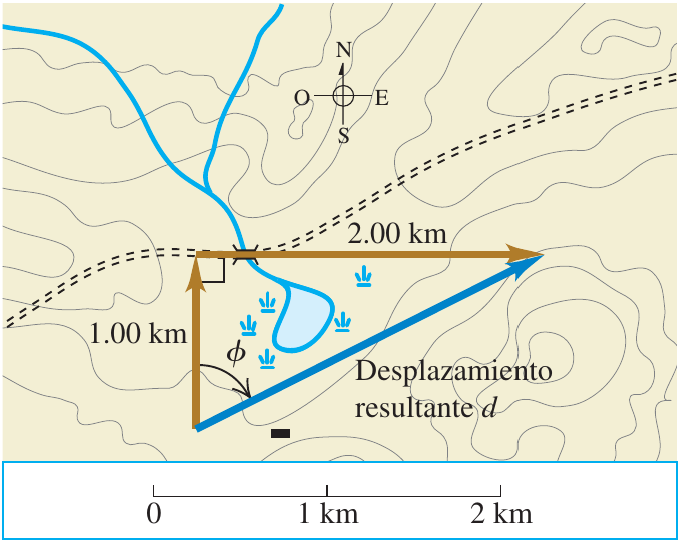
\includegraphics[scale=0.3]{figs/fig-03.png}
\end{center}

\cx
Una esquiadora de fondo viaja \qty{1.00}{km} al norte y luego \qty{2.00}{km} al este por un campo nevado horizontal. ¿A qué distancia y en qué dirección está con respecto de su punto de partida?
\pause
\vspace{1em}

Teorema de Pitágoras:
\[ \sqrt{(\qty{1.00}{km})^2 + (\qty{2.00}{km})^2} = \qty{2.24}{km} \]

Trigonometría simple:
\begin{align*}
    \tan \phi &= \frac{\qty{2.00}{km}}{\qty{1.00}{km}} \\
    \phi &= \ang{63.4}
\end{align*}
\end{columns}
\end{frame}

\begin{frame}{Componentes de vectores}
\begin{center}
    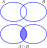
\includegraphics[scale=0.7]{figs/fig-03}
\end{center}
\begin{columns}
\cw{0.75}
\begin{itemize}
    \item $\hat{\bm{i}}$ es el vector unitario o \textbf{versor} en la dirección $x$, $\hat{\bm{j}}$ es el versor en la dirección $y$.
    \item $\vect{a}_x = a_x \, \hat{\bm{i}}, \, \vect{a}_y = a_y \, \hat{\bm{j}}$. $a_x$ y $a_y$ son las \textbf{componentes} (escalares) del vector $\vect{a}$.
    \item $\vect{a} = \vect{a}_x + \vect{a}_y = a_x \hat{\bm{i}} + a_y \hat{\bm{j}}$
    \item $a_x = \norm{\vect{a}} \cos \phi; \, a_y = \norm{\vect{a}} \sin \phi \mapsto \norm{\vect{a}} = \sqrt{a_x^2 + a_y^2}, \phi = \arctan(a_y / a_x)$.
    \item \textbf{Suma:} $\vect{a} + \vect{b} = (a_x + b_x) \hat{\bm{i}} + (a_y + b_y) \hat{\bm{j}}$
\end{itemize}
\cw{0.30}
\begin{center}
    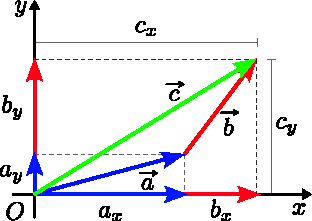
\includegraphics[width=1.0\textwidth]{figs/fig-04.pdf}
\end{center}
\end{columns}
\end{frame}

\begin{frame}{Componentes de vectores: ejemplos}
\begin{columns}
\cw{0.4}
\begin{center}
    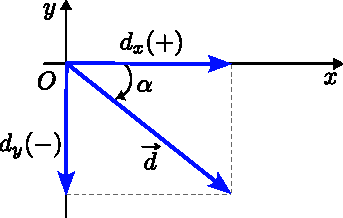
\includegraphics[width=0.75\textwidth]{figs/fig-05.pdf}
\end{center}
\cw{0.6}
\textbf{Ejemplo 1.} ¿Cuáles son las componentes $x$ y $y$ del vector $\vect{d}$? La magnitud del vector es $d = \qty{3.00}{m}$ y el ángulo es $\alpha = \ang{45}$.
\pause

\begin{align*}
    d_x = d \cos (\alpha) = (\qty{3.00}{m}) [\cos (\ang{-45})] = + \qty{2.1}{m} \\
    d_y = d \sen (\alpha) = (\qty{3.00}{m}) [\sen (\ang{-45})] = - \qty{2.1}{m}
\end{align*}
\end{columns}
\pause

\begin{columns}
\cw{0.4}
\begin{center}
    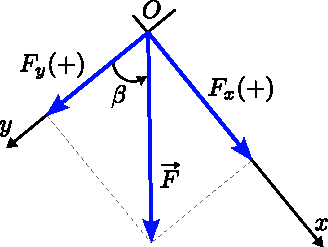
\includegraphics[width=0.75\textwidth]{figs/fig-06.pdf}
\end{center}
\cw{0.6}
\textbf{Ejemplo 2.} ¿Cuáles son las componentes $x$ y $y$ del vector $\vect{F}$? La magnitud del vector es $F = \qty{4.50}{m}$ y el ángulo es $\beta = \ang{37.0}$.
\pause

\begin{align*}
    F_x = F \sen (\beta) = (\qty{4.50}{m}) (\sen \ang{37.0}) = + \qty{2.71}{m} \\
    F_y = F \cos (\beta) = (\qty{4.50}{m}) (\cos \ang{37.0}) = + \qty{3.59}{m} \\
\end{align*}
\end{columns}
\end{frame}

\begin{frame}{Productos de vectores}
\begin{center}
    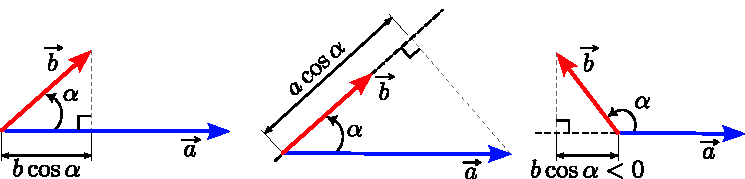
\includegraphics[width=0.75\textwidth]{figs/fig-07.pdf}
\end{center}
\begin{columns}[t]
\cx
\begin{definition}[Producto escalar]
    El \textbf{producto escalar}, \textbf{producto interno} o \textbf{producto punto} es una operación algebraica que toma dos vectores y retorna un escalar:
    \begin{align*}
        \vect{a} \cdot \vect{b} &= a \, b \, \cos \alpha \\
        \vect{a} \cdot \vect{b} &= a_x b_x + a_y b_y 
    \end{align*}
\end{definition}
\pause

\cx
\textbf{Nota 1:}
\begin{align*}
    \hat{\bm{i}} \cdot \hat{\bm{i}} &= \hat{\bm{j}} \cdot \hat{\bm{j}} = \hat{\bm{k}} \cdot \hat{\bm{k}} = (1)(1) \cos \ang{0} = 1 \\ 
    \hat{\bm{i}} \cdot \hat{\bm{j}} &= \hat{\bm{i}} \cdot \hat{\bm{k}} = \hat{\bm{j}} \cdot \hat{\bm{k}} = (1)(1) \cos \ang{90} = 0
\end{align*}
\textbf{Nota 2:}
\begin{multicols}{2}
\begin{itemize}
    \item $\vect{a} \cdot \vect{b} = \vect{b} \cdot \vect{a}$
    \item $\vect{a} \cdot \vect{a} \geq 0$
    \item $\norm{\vect{a}} = \sqrt{\vect{a} \cdot \vect{a}}$
    \item $\abs{\vect{a} \cdot \vec{b}} \leq \norm{\vect{a}} \cdot \norm{\vect{b}} $
\end{itemize}
\end{multicols}
\end{columns}
\end{frame}

\begin{frame}{Productos de vectores}
\begin{columns}
\cx
\begin{center}
    \includesvg[scale=0.5]{figs/mano_derecha.svg}
\end{center}

\begin{definition}[Producto vectorial]
    El \textbf{producto vectorial} o \textbf{producto cruz} es una operación entre dos vectores cuyo resultado es un vector \textbf{perpendicular} a los vectores que se multiplican. Si $\vect{a}, \vect{b} \in \mathbb{R}^3$:
    \[ \vect{a} \mul \vect{b} = (\norm{\vect{a}}\,\norm{\vect{b}}\, \sen \alpha) \hat{\bm{n}} \]
    donde $\hat{\bm{n}}$ es un versor perpendicular a $\vect{a}$ y $\vect{b}$ cuyo sentido está dado por la regla de la mano derecha.
\end{definition}
\pause

\cx
\textbf{Cálculo con componentes:}
\[ \vect{a} \mul \vect{b} =
    \begin{vmatrix}
        \hat{\bm{i}} & \hat{\bm{j}} & \hat{\bm{k}} \\
        a_x & a_y & a_z \\
        b_x & b_y & b_z
    \end{vmatrix} \]
\pause

\textbf{Algunas propiedades:}
\begin{itemize}
    \item $(\vect{a} \mul \vect{b}) \mul \vect{c} \neq \vect{a} \mul (\vect{b} \mul \vect{c})$ \textbf{No} es asociativo.
    \item $\vect{a} \mul \vect{b} = -(\vect{b} \mul \vect{a})$ Anticonmutativo.
    \item Si $\vect{a} \mul \vect{b} = 0, \vect{a} \neq \vect{0}$ y $\vect{b} \neq \vect{0}$, entonces $\vect{a} \, \parallel \, \vect{b}$.
    \item $\vect{a} \cdot (\vect{a} \mul \vect{b}) = 0$
    \item $(\vect{a} + \vect{b}) \mul \vect{c} = \vect{a} \mul \vect{c} + \vec{b} \mul \vect{c}$
    \item $\vect{a} \mul (\vect{b} \mul \vect{c}) = \vect{b}(\vect{a} \cdot \vect{c}) - \vect{c} (\vect{a} \mul \vect{b})$
\end{itemize}
\end{columns}
\end{frame}



\end{document}

